\documentclass[tikz]{standalone}
\usepackage{pgfplots}
\pgfplotsset{compat=1.15}
\usepackage{mathrsfs}
\usetikzlibrary{arrows,calc}
\usepackage{tkz-euclide}
\pagestyle{empty}

\definecolor{AngleClr}{rgb}{0,0.39215686274509803,0}
\definecolor{ShapeClr}{rgb}{0.6,0.2,0}
\definecolor{SquareClr}{RGB}{250, 248, 217}

\usepackage{fp}
\usepackage{xfp}

\begin{document}

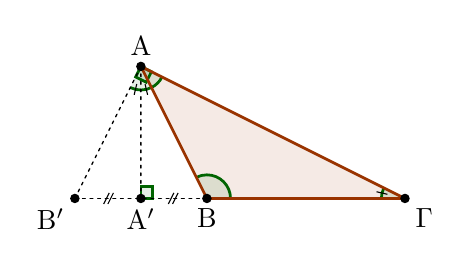
\begin{tikzpicture}[scale=.75]
\tkzSetUpLine[line width=1pt,color=black]
\tkzSetUpPoint[fill=black]

\def\Scale{2.5}
\def\La{1 * \Scale}
\def\Lb{2 * \Scale}
\def\Lc{\fpeval{sqrt(\La * \La + \Lb * \Lb)}}

\FPeval{\Ax}{\La * \La / \Lc}
\FPeval{\Ay}{\La * \Lb / \Lc}

\tkzDefPoints{0/0/B,\Ax/\Ay/A,\Lc/0/C}


\tkzDefPointBy[projection=onto B--C](A)\tkzGetPoint{H}

\tkzDefPointsBy[symmetry=center H](B){}

\tkzFillPolygon[fill=ShapeClr,fill opacity=0.1](A,B',C)
\tkzFillAngle[fill=AngleClr,size=.4,fill opacity=0.1](C,B',A)
\tkzMarkAngle[line width=1pt,size=.4,color=AngleClr](C,B',A)

\tkzFillAngles[fill=AngleClr,size=.4,fill opacity=0.1](A,C,B B,A,H H,A,B')
\tkzMarkAngles[mark=|, mksize=2, line width=1pt,color=AngleClr,size=.4](A,C,B B,A,H H,A,B')

\tkzFillAngle[fill=AngleClr,size=.4,fill opacity=0.1](B',A,C)
\tkzMarkAngle[line width=1pt,color=AngleClr,size=.4](B',A,C)
\tkzMarkRightAngles[line width=1pt, size=.2,color=AngleClr,fill=AngleClr,fill opacity=0.1](A,H,B' B,A,C)

\tkzDrawPolygon[color=ShapeClr](A,B',C)

\tkzDrawPoints[size=3](A,B,C,H,B')

\tkzDrawSegments[line width=0.5pt,color=black,dashed,dash pattern=on 1pt off 1.75pt](B,B' B,A H,A)

\tkzMarkSegments[mark=s||,size=2](B,H B',H)

\tkzLabelPoint[above](A){$\rm A$}
\tkzLabelPoint[below left](B){$\rm B'$}
\tkzLabelPoint[below](B'){$\rm B$}
\tkzLabelPoint[below](H){$\rm A'$}
\tkzLabelPoint[below right](C){$\rm \Gamma$}

\end{tikzpicture}

\end{document}
